\apendice{Documentación técnica de programación}

\section{Introducción}

La documentación técnica de programación describirá la estructura de los programas empleados en el proyecto, el entorno de desarrollo, la instalación y ejecución de los programas.

\section{Estructura de directorios}

Dentro de GitLab tendremos programas y códigos que nos resultaran ajenos para el correcto funcionamiento, estos programas son pruebas realizadas anteriormente (tutoriales, código de pruebas \ldots).

Para el desarrollo del proyecto \footnote{Repositorio GitLab: \url{https://gitlab.com/HP-SCDS/Observatorio/2018-2019/ubu-bc4distribution/tree/paginaWeb}} \footnote{Repositorio GitHub: \url{https://github.com/ers0026/ProyectoFinal}}, se utiliza los siguientes ramas:

\begin{itemize}
	\item \textit{Proyecto}: en la raíz \textbackslash xampp\textbackslash htdocs\textbackslash proyectoFinal tendremos todo el contenido del código de nuestro proyecto, archivos: PHP, CSS, Bootstrap \ldots y también el enlace de conexión con metamask.
	\item \textit{Documentación}: se encontrará en la carpeta Latex y contará con la documentación (memoria y anexos) para la compresión del funcionamiento de la aplicación, también cuenta con un guion de la instalación de truffle, el cual no hace falta para el funcionamiento pero creemos que un buena herrmienta para el funcionamiento del proyecto). También se dispondrán los pdf en la rama principal para su fácil acceso.
\end{itemize}

\section{Manual del programador}

En esta sección hablaremos de la instalación de los programas necesarios para el funcionamiento de la página web y su conexión con la red Ethereum.

\begin{itemize}
	\item \textbf{Metamask\label{ref:install}} 
	\begin{itemize}
		\item Primeramente realizaremos la instalación en el navegador que deseemos desde la página\footnote{\url{https://metamask.io/}} (en nuestro caso lo hemos realizado desde Google Chrome).
		\item Ahora nos redireccionará y nos aparecerá un botón ``Añadir a Chrome''. 
		\item A continuación nos saldrá una pantalla emergente: ``Añadir extensión''. 
		\item Esto instalará en la barra de extensiones el símbolo de metamask, un zorro. 
	\end{itemize}

Después de estos pasos, tendremos una serie de pasos a realizar para importar la cuenta:
	
	\begin{itemize}
		\item Primera imagen indica el comienzo de metamask \ref{fig:Metamask1}, pulsaremos ``\textit{Get Started}'' para continuar.
		\item Seguidamente tendremos dos caminos posibles \ref{fig:Metamask2}:
			\begin{enumerate}
				\item Continuar con una cuenta ya existente.
				\item Crear una nueva cuenta.
			\end{enumerate}
		En este caso iremos por el camino de ``\textit{Importar Wallet}'' ya que las operaciones las realizaremos desde la misma cuenta, si deseáramos cambiar de cuenta tendríamos que realizar cambios en el código.	
		\item A continuación, nos pedirá los permisos para analizar los movimientos que realizamos, pulsaremos ``\textit{I agree}''\ref{fig:Metamask3}
		\item Esta es la pantalla más importante, ya que tendremos que tener la cadena de palabras \textit{nmonic} que nos dieron al crear la cuenta por primera vez y al iniciar en otro ordenador tendremos que introducir nuevamente una contraseña para entrar futuras veces (pondremos la misma contraseña que tenemos en otros navegadores o equipos) para así tener acceso siempre a nuestro metamask y aceptaremos los terminos de uso. Una vez todo este realizado pulsaremos ``importar'' \ref{fig:Metamask4}
		\item Nos mostrará un mensaje de registro completado con exito \ref{fig:Metamask5} y tendremos que clic en ``All done''
	\end{itemize}
	
\begin{figure}[H]
	\begin{minipage}[b]{0.5\linewidth}
		\centering
		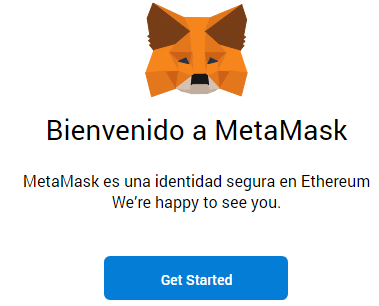
\includegraphics[width=\linewidth]{Metamask1}
		\caption{Confirmar el contrato}
		\label{fig:Metamask1}
	\end{minipage}
\hspace{0.5cm}
	\begin{minipage}[b]{0.5\linewidth}
		\centering
		\includegraphics[width=\linewidth]{Metamask2}
		\caption{Conexión pendiente}
		\label{fig:Metamask2}
	\end{minipage}
	\begin{minipage}[b]{0.5\linewidth}
		\centering
		\includegraphics[width=\linewidth]{Metamask3}
		\caption{Confirmar el contrato}
		\label{fig:Metamask3}
	\end{minipage}
\hspace{0.5cm}
	\begin{minipage}[b]{0.5\linewidth}
		\centering
		\includegraphics[width=\linewidth]{Metamask4}
		\caption{Conexión pendiente}
		\label{fig:Metamask4}
	\end{minipage}
	\begin{minipage}[b]{0.8\linewidth}
		\centering
		\includegraphics[width=\linewidth]{Metamask5}
		\caption{Conexión confirmada}
		\label{fig:Metamask5}
	\end{minipage}
\end{figure}

		
	\item \textbf{XAMPP}
	
Para descargar el programa XAMPP, tendremos que seguir los siguientes pasos:	
	\begin{enumerate}
		\item Iremos a la página\footnote{\url{https://www.apachefriends.org/index.html}}.
		\item Elegiremos la versión en la que ejecutaremos XAMPP (Windows, Linux o iOS.
		\item Una vez descargado, buscaremos el archivo ``xampp-win32-7.2.4-0-VC15-installer'' y ejecutaremos el archivo.
		\item Cuando se abra la primera pantalla, haremos clic en \textit{Yes}.
		\item A continuación seleccionaremos las funciones XAMPP que deseamos instalar, en nuestro caso seleccionamos todas ellas, será la forma predeterminada y pulsaremos ``\textit{Next}''.
		\item Seleccionaremos la ubicación donde deseemos instalar el programa. Una vez ubicado pulsaremos ``\textit{Next}''.
		\item En la penúltima pantalla desmarcaremos la opción de ``textit{Learn more about Bitnami for XAMPP}'' ``Aprender más sobre Bitnami'' y clicamos ``\textit{Next}''.
		\item Con esto empezará a instalar XAMPP en la carpeta seleccionada. Pulsaremos \textit{Finish}, esto cerrará la ventana y abrirá el panel de control de XAMPP y aquí accedemos a los servidores. Antes de ello, tendremos que seleccionar el idioma que deseemos. 
	\end{enumerate}	
	\item \textbf{Visual Stuido Code}
	\begin{enumerate}
		\item Nos dirigiremos a la página\footnote{\url{https://code.visualstudio.com/}} y seleccionaremos para qué sistema deseamos el programa: Windows, Linux, macOS.
		\item Una vez descargado, se abrirá un asistente de instalación y tendremos que aceptar el acuerdo de licencia y pulsaremos ``siguiente''.
		\item Elegiremos la carpeta donde instalará el programa.
		\item La siguiente pantalla nos preguntara sobre las tareas adicionales que queremos realizar, una vez seleccionadas pulsaremos siguiente.
		 \item La penúltima pantalla, clicaremos sobre ``instalar''. Una vez finalizado nos preguntará si deseamos ejecutarle por primera vez y pulsaremos ``finalizar''.
		 \item  Ahora, cada vez que queremos iniciar el programa, sólo tendremos que pulsar sobre el icono creado de Visual Studio Code para iniciar el programa. 
	\end{enumerate}	
\end{itemize}

\section{Compilación, instalación y ejecución del proyecto}\label{intalacionE}

\subsection{Descarga del proyecto}
En este apartado explicáramos los pasos a realizar para poder tener la aplicación web en nuestro ordenador y poder coger la base de datos y poder operar con ella directamente. 

Para la obtención del código \cite{GitLab} \cite{GitHub} y los recursos del proyecto, tendremos que dirigirnos al repositorio desde el siguiente enlace\footnote{Repositorio GitLab: \url{https://gitlab.com/HP-SCDS/Observatorio/2018-2019/ubu-bc4distribution/tree/paginaWeb}} \footnote{Repositorio GitHub: \url{https://github.com/ers0026/ProyectoFinal}}.

Tendremos que descargar la carpeta XAMPP, primeramente habrá que descomprimirlo y guardarlo directamente en (C:), seguidamente dentro de la carpeta XAMPP encontraremos diferentes carpetas y documentos:

\begin{enumerate}
	\item En dicha carpeta buscaremos el archivo \textbf{xampp\_start.exe} \ref{fig:figura11}, clicaremos sobre ese ejecutable, a continuación daremos los permisos pertinentes para poder ejecutar el archivo.
	\item Con esto se activaran los módulos de Apache y MySQL. Para cerciorarnos que están activados tendremos que ejecutar \textbf{xampp\_control.exe} \ref{fig:figura11} y ejecutar desde los comandos \textit{START} de Apache y MySQL que tenemos en fosforito en la imagen \ref{fig:figura12}.
\end{enumerate}

\begin{figure}[h!]
	\centering
	\begin{minipage}[b]{0.8\linewidth}
		\centering
		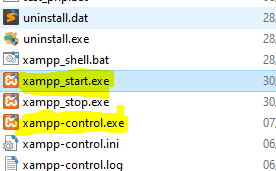
\includegraphics[width=\linewidth]{XAMPPautomatico}
		\caption{Ejecución de XAMPP automáticamente}
		\label{fig:figura11}
	\end{minipage}
	\begin{minipage}[b]{0.8\linewidth}
		\centering
		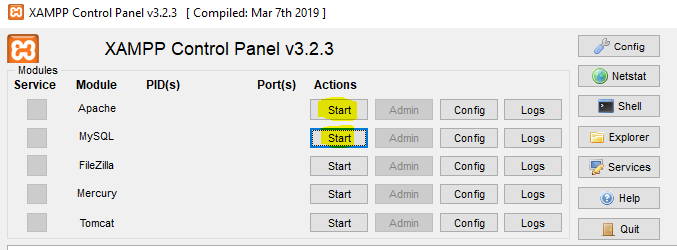
\includegraphics[width=\linewidth]{XAMPPmanual}
		\caption{Ejecución de XAMPP manualmente}
		\label{fig:figura12}
	\end{minipage}
\end{figure}


Así ya tendremos nuestra base de datos local activada y tendremos que dirigirnos a nuestro navegador para poner en nuestro navegador: localhost/proyectoFinal (proyectoFinal, ya que es así como se llama la carpeta donde tenemos el código de la página web).

Una vez estemos visualizando la página web en el modo local, nos servirá de ayuda el punto Interfaz gráfica \textit{Front-End} \ref{ref:front}

Una vez descargado el archivo y tengamos acceso a la página web tendremos que instalar Metamask \ref{ref:install}

Metamask: tendremos que estar registrados previamente o, si no, al añadir producto nos saldrá una pantalla para introducir la contraseña\footnote{La contraseña la tendremos en un archivo en el GitLab y GitHub, el archivo se llama nemonic metamask.txt} y a continuación nos desplegará el primer contrato. Para comenzar a funcionar tendremos que  seleccionar la Red privada Ropsten.
